\documentclass[a4paper,12pt]{article}
\usepackage{amsmath}  % For equations
\usepackage{amsfonts} % For mathematical symbols
\usepackage{graphicx} % For figures
\usepackage{hyperref} % For links
\usepackage{appendix} % For appendices
\usepackage [round,authoryear] {natbib}
\usepackage{float}

\DeclareMathOperator*{\argmax}{argmax}
\DeclareMathOperator*{\argmin}{argmin}

\usepackage{amsthm}
\usepackage{xcolor}

\theoremstyle{definition}
\newtheorem{exinn}{Example}

\newenvironment{example}
{\clubpenalty=10000
	\begin{exinn}%
		\mbox{}%
		{\color{black}\leaders\hrule height .8ex depth \dimexpr-.8ex+0.8pt\relax\hfill}%
		\mbox{}\linebreak\ignorespaces}
	{\par\kern2ex\hrule\end{exinn}}


\title{Bayesian Decision Theory\\
	\small{Median Decision Rule}}
\author{Jonas Petersen \\ Ander Runge Walther }
\date{\today}

\begin{document}
	\maketitle
	
	\begin{abstract}
		This study investigates the derivation of the median as the optimal decision rule from a specific cost function within the framework of Bayesian decision theory. By exploring the implications of a linear asymmetric cost function, we illustrate the skewness in penalty structures associated with underestimation and overestimation. The analysis leads to the formulation of an expected cost that highlights the importance of the median in decision-making scenarios.
	\end{abstract}
	
	\noindent
	This study considers how the median can be derived as the optimal decision rule from a particular cost function using Bayesian decision theory. Let $s$ denote the true value and $U(x,D)$ the estimate based on input $x$ and data $D$. A linear asymmetric cost function can be expressed viz
	\begin{equation}
		C(U(x,D), s) = \alpha \cdot \text{swish}(U(x,D) - s, \beta) + (1 - \alpha) \cdot \text{swish}(s - U(x,D), \beta)
		\label{eq:cost}
	\end{equation}
	where the function $\text{swish}(z,\beta)$ is defined as
	\begin{equation}
		\text{swish}(z,\beta) = \frac{z}{1 + e^{-z\beta}}.
	\end{equation}
	For brevity, we set $z \equiv U(x,D) - s$. When $\beta \gg 1$, equation \eqref{eq:cost} approximates two linear segments around the origin, as illustrated in Figure \ref{fig:1}.
	\begin{figure}[H]
		\centering
		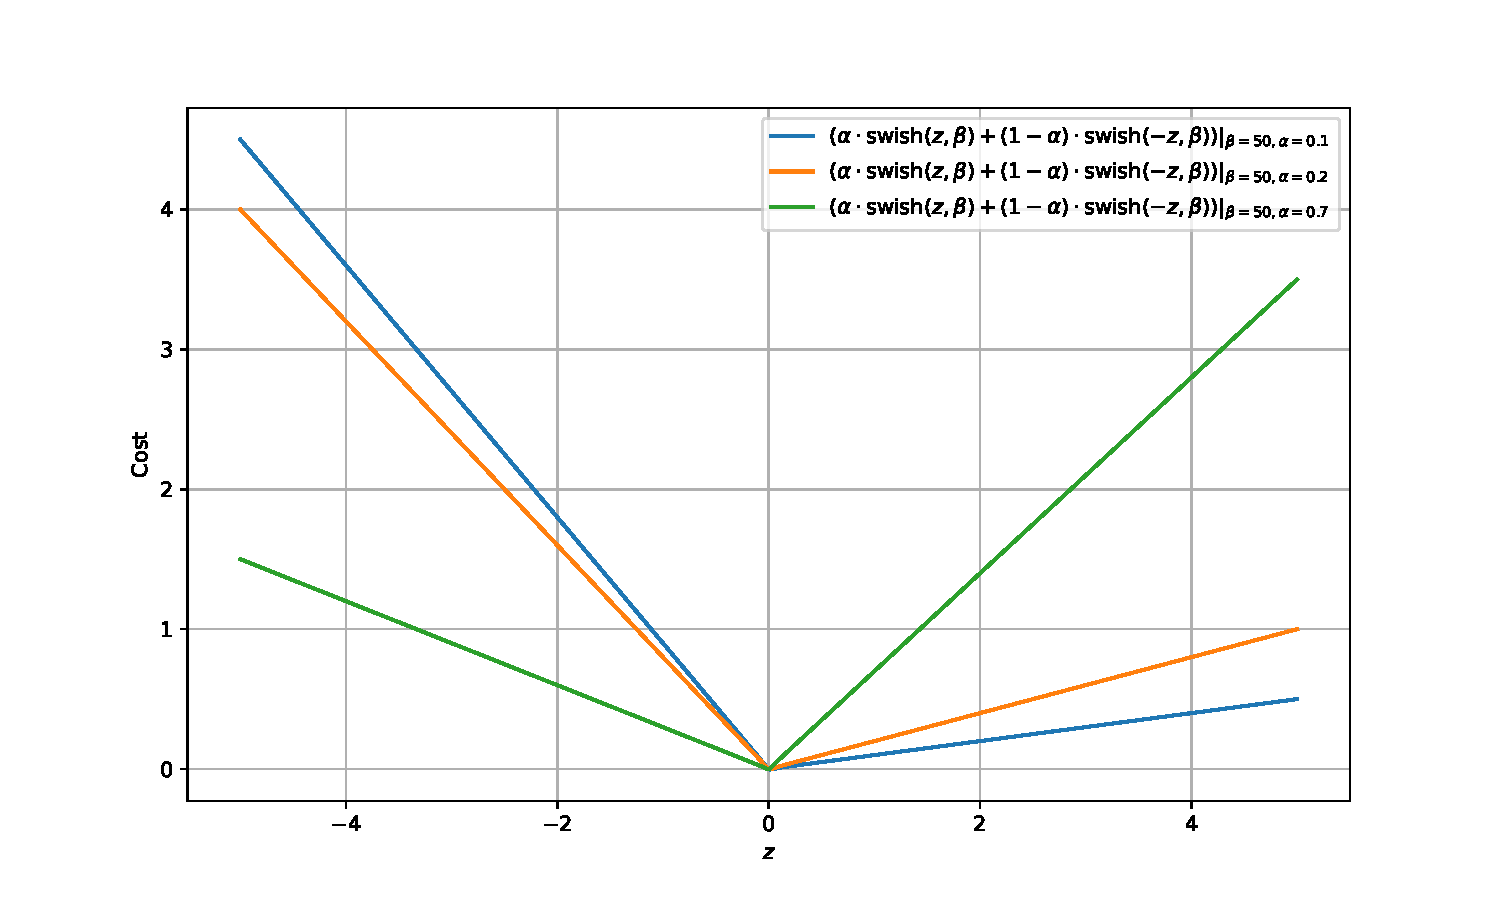
\includegraphics[width=1\textwidth]{figures/cost_plot.pdf}
		\caption{Illustration of equation \eqref{eq:cost} with different parameter values $\alpha$ and $\beta$.}
		\label{fig:1}
	\end{figure}
	By taking $\alpha \ll 1$, we observe that when $z < 0$ (indicating underestimation), the penalty incurred is relatively greater than for $z > 0$ (indicating overestimation). This skewed penalty structure emphasizes the greater cost associated with underestimating the true value.
	
	We can now compute the expected cost given the input and data as follows
	
	\begin{equation}
		\begin{split}
			\mathbb{E}[C | x, D, I] & = \int ds \, p(s | x, D, I) \bigg( \alpha \cdot \text{swish}(U(x,D) - s, \beta) \\
			& \quad + (1 - \alpha) \cdot \text{swish}(s - U(x,D), \beta) \bigg),
		\end{split}
		\label{eq:1}
	\end{equation}
	
	where $I$ denotes the background information~\citep{Sivia2006}. The optimal decision rule $U^*(x,D)$ can be found from the derivative
	\begin{equation}
		\begin{split}
			\frac{dC}{dU} & = \frac{dC}{dz}\frac{dz}{dU}\\
			& = \bigg(\frac{\alpha}{1+e^{-\beta z}}-\frac{1-\alpha}{1+e^{\beta z}}+\frac{\alpha\beta e^{-\beta z}z}{(1+e^{-\beta z})^2}+\frac{(1-\alpha)\beta e^{\beta z}z}{(1+e^{\beta z})^2}\bigg)\frac{dz}{dU}\\
			&= \frac{\beta z e^{\beta z}-e^{\beta z}-1}{(1+e^{\beta z})^2}+\alpha+\mathcal{O}(\alpha^2)\\
			&\approx  \alpha -\frac{1}{(1+e^{\beta z})^2}
		\end{split}
		\label{eq:2}
	\end{equation}
	where it has been used that $\alpha\ll 1$. Combining equations \eqref{eq:1} and \eqref{eq:2} alongside imposing the derivative vanish for the optimal decision rule
	\begin{equation}
		\begin{split}
			\frac{d\mathbb{E}[C|x,D,I ]}{dU}\bigg|_{U=U^*} &\approx \int ds p(s|x,D,I) \bigg(\alpha -\frac{1}{(1+e^{\beta z})^2}\bigg)\\
			& = \alpha -\int ds p(s|x,D,I)\frac{1}{(1+e^{\beta z})^2}\\
			& = 0
		\end{split}
	\end{equation}
	$\frac{1}{(1+e^{\beta z})^2}$ approximate a unit step which is $1$ for $z<0$ and $0$ otherwise. $z<0 \Rightarrow s>U(x)$. This means
	\begin{equation}
		\int_{-\infty}^{\infty} ds p(s|x,D,I)\frac{1}{(1+e^{\beta z})^2} \approx \int_{U^*}^{\infty} ds p(s|x,D,I)
	\end{equation}
	This means
	\begin{equation}
		\alpha \approx \int_{U^*}^{\infty} ds p(s|x,D,I)
		\label{eq:decision}
	\end{equation}
	which is the definition of a the $\alpha$-quantile. Figure \ref{fig:2} show how $\alpha$ and $U^*$ are related via equation \eqref{eq:decision} in graphical terms (the $\alpha$-quantile). Figure \ref{fig:3} show the relative difference between numerically optimizing the expected cost and the percentile, as a function of $\alpha$, for an arbitrary gamma distribution. Numerical imperfections aside, the figure shows that the two are identical. The code can be found in the src folder in the project directory.
	
	\begin{figure}[H]
		\centering
		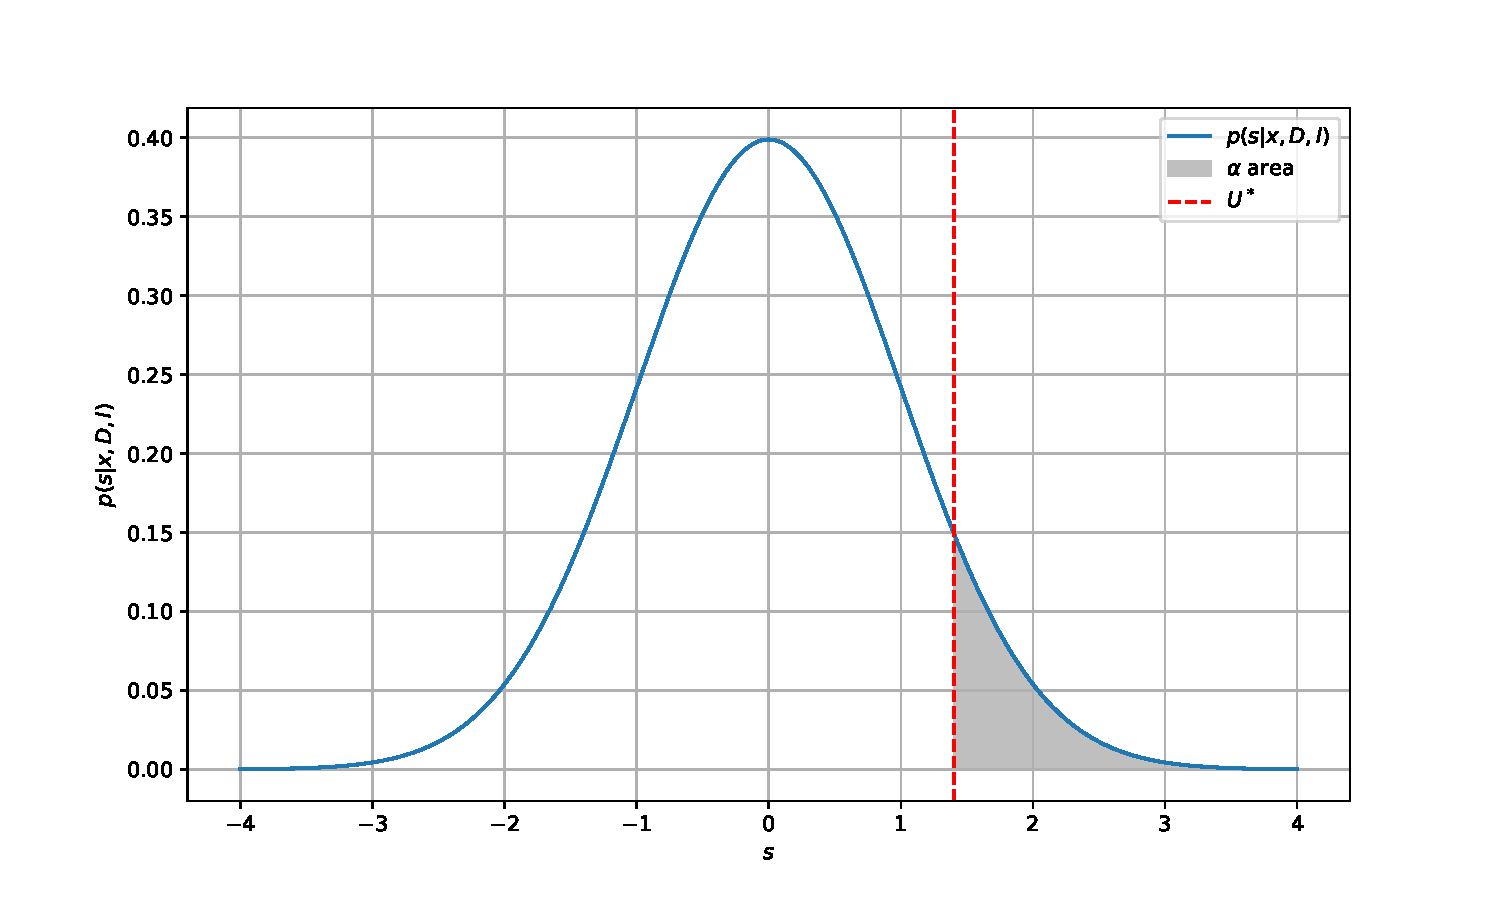
\includegraphics[width = 1\textwidth]{figures/alpha_plot.pdf}
		\caption{Illustration of equation \eqref{eq:decision} with $\alpha = 0.05$. A simple normal distribution has been used for illustrative purposes while it is understood equation \eqref{eq:decision} generalize beyond this simple setting.}
		\label{fig:2}
	\end{figure}
	\begin{figure}[H]
		\centering
		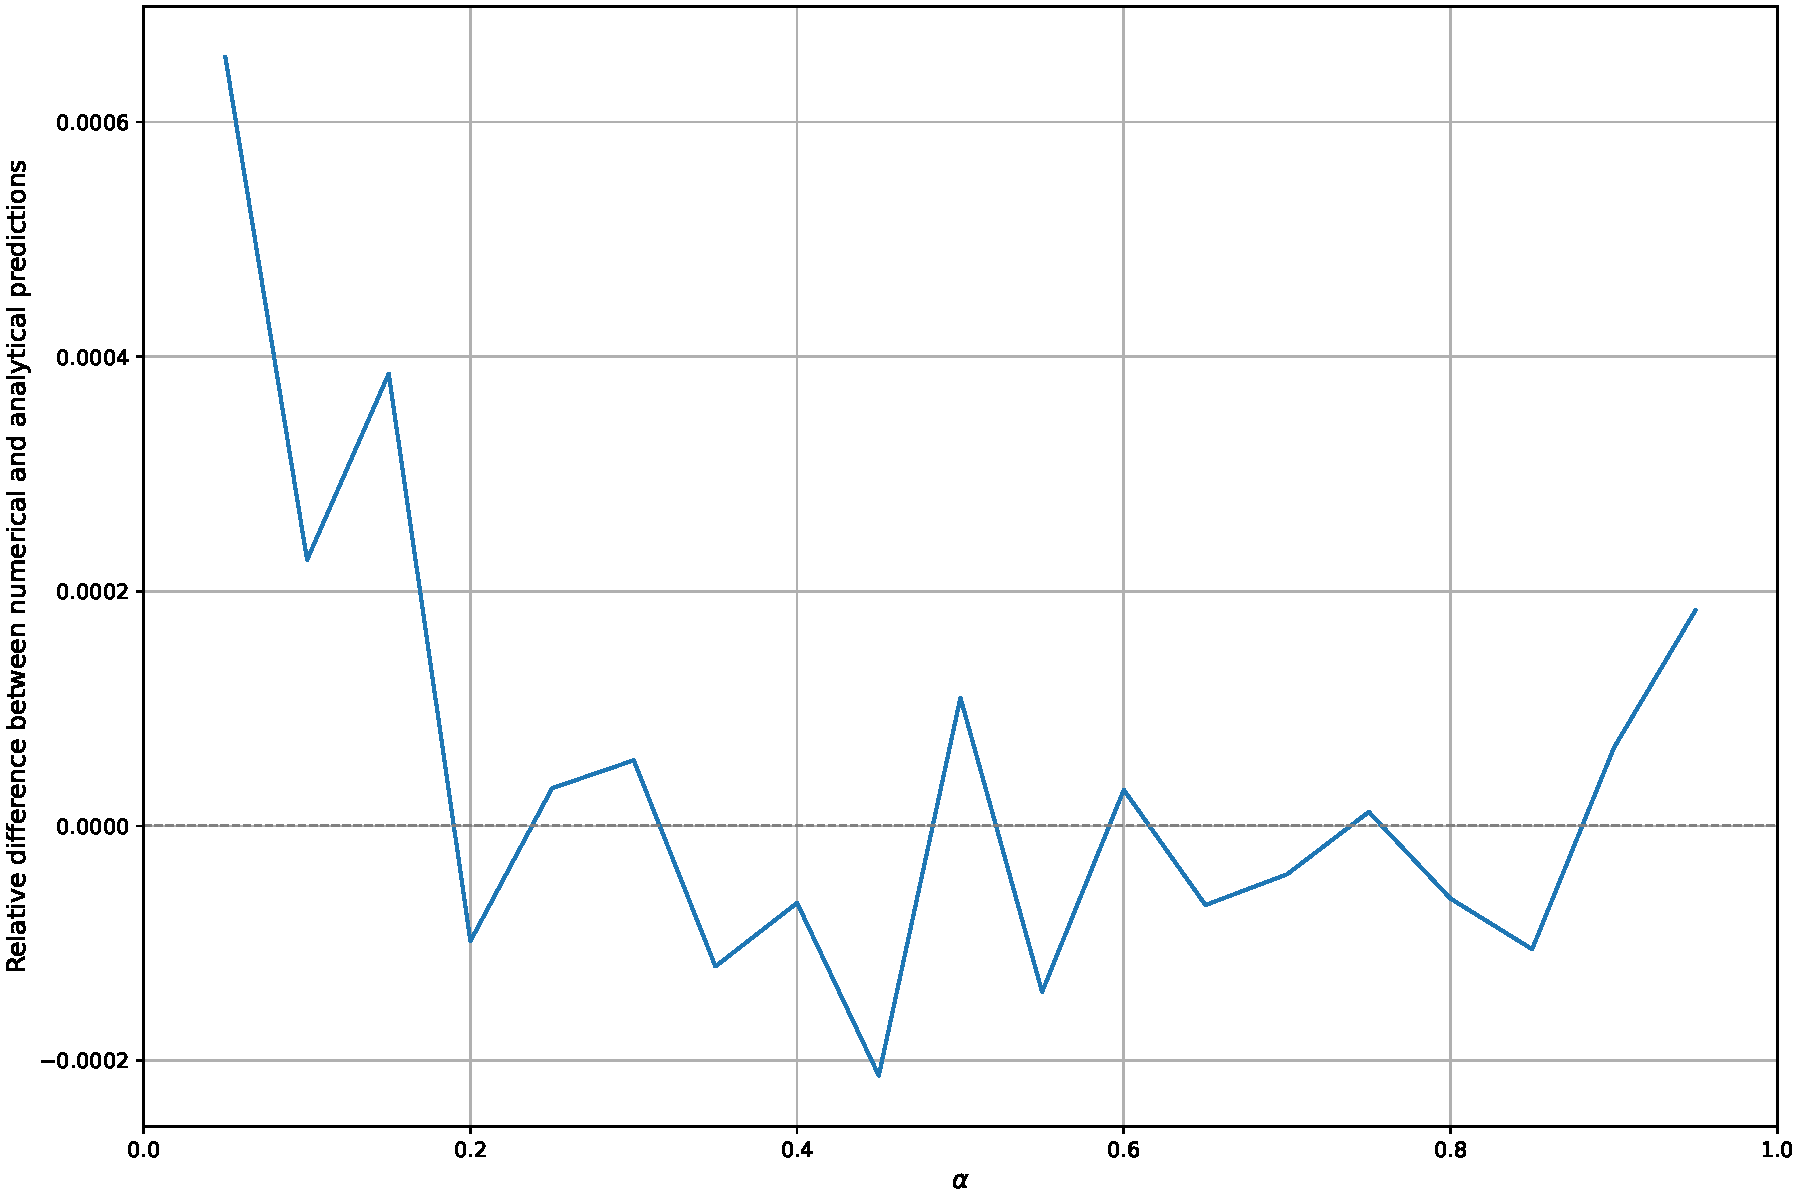
\includegraphics[width = 0.8\textwidth]{figures/numerical_example.pdf}
		\caption{The relative difference between numerically optimizing the expected cost and the percentile, as a function of $\alpha$.}
		\label{fig:3}
	\end{figure}
	
	
	\bibliographystyle{plainnat}
	\bibliography{ref}
	
\end{document}